%%%%%%%%%%%%%%%%%%%%%%%%%%%%%%%%%%%%%%%%%%%
% File      : annexe-orthotropie
% Author    : THOMAS HELFER
% Date      : 7 mer. 2012
% Directory : /home/th202608/codes/MFrontMaterials/trunk/src/trunk/docs/description
%%%%%%%%%%%%%%%%%%%%%%%%%%%%%%%%%%%%%%%%%%%

\section{Rappels sur les lois de comportement orthotropes et application
  aux tubes}
\label{sec:annexe:orthotropie}

Un matériau (mécaniquement) orthotrope possède, en chaque point
d'espace, trois plans de symétrie ortho\-gonaux vis à vis de son
comportement mécanique. Ces trois plans définissent trois directions
perpendiculaires appelées directions d'ortho\-tropie.

Un repère d'orthotropie est un repère orthonormé formé par ces trois
directions. Le problème traité amène souvent à privilégier un de ces
repères pour décrire le comportement mécanique du matériau. Le cas des
tubes sera par exemple traité en détails au
paragraphe~\ref{sec:conv-de-rang}. Le repère est alors appelé le repère
d'orthotropie du matériau. Les trois directions associées à ce repère
sont simplement notées \(1\), \(2\) et \(3\). {\em Dans la suite,
  l'expression de la loi de comportement mécanique, de la matrice de
  souplesse et des différents tenseurs, se fera toujours dans ce
  repère.}

\subsection{Directions d'orthotropie}
\label{sec:orthotropie}

Le tenseur des  contraintes sera dans la suite représenté sous forme
vectorielle. En \(3D\), ce tenseur s'écrira donc~:
\begin{equation}
  \label{eq:tsigma}
  \tsigma = \left(
    \begin{array}{c}
      \sigma_{11} \\
      \sigma_{22}  \\
      \sigma_{33}  \\
      \sqrt{2}\,\sigma_{12} \\
      \sqrt{2}\,\sigma_{13} \\
      \sqrt{2}\,\sigma_{23} \\
    \end{array}
  \right)
\end{equation}

De même, le tenseur des déformations totales sera représenté par le
vecteur suivant~:
\begin{equation}
  \label{eq:tepsilonto}
  \tepsilonto = \left(
    \begin{array}{c}
      \epsilonto_{11} \\
      \epsilonto_{22}  \\
      \epsilonto_{33}  \\
      \sqrt{2}\,\epsilonto_{12} \\
      \sqrt{2}\,\epsilonto_{13} \\
      \sqrt{2}\,\epsilonto_{23} \\
    \end{array}
  \right)
\end{equation}

Contrairement aux notations de \nom{Voigt} utilisées par le code aux
éléments finis \castem{}, ces notations permettent de symétriser le
rôle des contraintes et des déformations et de substituer au produit
doublement contracté de deux tenseurs le produit scalaire de leurs
représentations vectorielles. Cette symétrie des tenseurs des
contraintes et de déformations est particulièrement utile quand des
calculs tensoriels complexes sont nécessaires.

Notons que l'ordre des composantes de cisaillement n'est pas celui des
notations de \nom{Voigt}, mais reprend celui utilisé par le code aux
éléments finis \castem{}.

\subsection{Élasticité}
\label{sec:elasticite}

Dans le cadre de l'élasticité linéaire, les contraintes $\tsigma$ sont
liées aux déformations élastiques $\tepsilonel$ par la {\bf matrice de
  rigidité}, appelée également {\bf matrice d'élasticité} dans la
suite et notée $\tenseurq{D}$, ou par son inverse, la {\bf matrice de
  souplesse}, notée $\tenseurq{S}$, par la relation~:
\[
\tsigma=\tenseurq{D}:\tepsilonel
,\quad\text{et}\quad
\tepsilonel=\tenseurq{S}:\tsigma
.\]

La matrice de souplesse d'un matériau orthotrope s'écrit, dans le
repère d'orthotropie, sous la forme~:
\begin{equation}
  \label{eq:S}
  \tenseurq{S}=
  \begin{pmatrix}
    \Frac{1}{E_1}&-\Frac{\nu_{12}}{E_1}&-\Frac{\nu_{13}}{E_1}&0&0&0\\
    -\Frac{\nu_{21}}{E_2}&\Frac{1}{E_2}&-\Frac{\nu_{23}}{E_2}&0&0&0\\
    -\Frac{\nu_{31}}{E_3}&-\Frac{\nu_{32}}{E_3}&\Frac{1}{E_3}&0&0&0\\
    0&0&0&\Frac{1}{2\,G_{12}}&0&0\\
    0&0&0&0&\Frac{1}{2\,G_{13}}&0\\
    0&0&0&0&0&\Frac{1}{2\,G_{23}}\\
  \end{pmatrix}
\end{equation}
Elle est donc caractérisée par \(9\) coefficients indépendants~:
\begin{itemize}
\item \(3\) modules d'\nom{Young} $E_1$, $E_2$ et $E_3$~;
\item \(3\) coefficients de \nom{Poisson} $\nu_{12}$, $\nu_{13}$ et
  $\nu_{23}$~;
\item \(3\) modules de cisaillement $G_{12}$, $G_{13}$ et $G_{23}$.
\end{itemize}

Le facteur \(2\) apparaissant sur les modules de cisaillement est dû à
la convention de représentation des tenseurs utilisée dans cette note
(paragraphe~\ref{sec:orthotropie}) et est introduit pour que la
définition des modules d'élasticité soit cohérente avec les conventions
\castem{} qui utilise une notation proche de celle de \nom{Voigt}. En
particulier, les termes de cisaillement s'écrivent~:
\[
\sigma_{12} = 2\,G_{12}\epsilonel_{12}
\]

Les trois coefficients de Poisson, $\nu_{21}$, $\nu_{31}$ et
$\nu_{32}$ vérifient les relations imposées par la symétrie de la
matrice $\tenseurq{S}$~:
\[
\nu_{21}=\Frac{E_2}{E_1}\,\nu_{12}
,\quad
\nu_{31}=\Frac{E_3}{E_1}\,\nu_{13}
\quad\text{et}\quad
\nu_{32}=\Frac{E_3}{E_2}\,\nu_{23}
,\]

\subsection{Critère de \nom{Hill}}
\label{sec:critere-de-nomhill}

Par analogie avec l'usage courant pour les matériaux isotropes et en
accord avec l'expérience, la plupart des écoulements plastiques ou
viscoplastiques sont décrits en introduisant une variable scalaire de
l'état des contraintes, la contrainte équivalente de \nom{Hill}, notée
dans la suite \(\sigmaH\)~\cite{cha_1996,caill_98}. L'intensité de
l'écoulement est fonction de cette contrainte équivalente et les
composantes du tenseur des contraintes n'interviennent pas
explicitement.

Bien que cela ne soit pas nécessaire, nous ferons dans la suite
l'hypothèse de normalité de l'écoulement~: la direction d'écoulement
est donnée par la normale aux iso-surfaces de la contrainte
équivalente.

\paragraph{Tenseur de Hill}

Avant de donner l'expression de la contrainte équivalente, il est
pratique d'introduire un tenseur d'ordre \(4\), nommé dans la suite
tenseur de \nom{Hill} et noté \tenseurq{H}~:
\begin{equation}
  \label{eq:H}
  \tenseurq{H} =
  \left(
    \begin{array}{cccccc}
      F+H & -F  & -H  & 0 & 0 & 0 \\
      -F  & G+F & -G  & 0 & 0 & 0 \\
      -H  & -G  & H+G & 0 & 0 & 0 \\
      0   & 0   & 0   & L & 0 & 0 \\
      0   & 0   & 0   & 0 & M & 0 \\
      0   & 0   & 0   & 0 & 0 & N \\
    \end{array}
  \right)
\end{equation}
où les \(6\) coefficients \(F\), \(G\), \(H\), \(L\), \(M\) et \(N\)
doivent être identifiés expérimentalement.

\paragraph{Contrainte équivalente au sens de \nom{Hill}}

La contrainte équivalente au sens de \nom{Hill} s'écrit
classiquement~:
\[
\sigmaH = \sqrt{\tsigma\colon\,\tenseurq{H}\colon\, \tsigma}
\]

En développant cette expression avec les conventions d'écriture du
tenseur des contraintes décrites par l'équation~\eqref{eq:tsigma},
nous obtenons~:
\begin{equation}
  \label{eq:sigH}
  \sigmaH = \sqrt{\left(\sigma_{22}-\sigma_{11}\right)^2\,F +
    \left(\sigma_{33}-\sigma_{22}\right)^2\,G +
    \left(\sigma_{11}-\sigma_{33}\right)^2\,H +
    2\,\sigma_{12}^2\,L +
    2\,\sigma_{13}^2\,M +
    2\,\sigma_{23}^2\,N}
\end{equation}

\paragraph{Tenseur normal} Le tenseur normal \(\tenseur{n}\) est
défini comme la normale aux iso-surfaces de la contrainte équivalente.
Il est donc égal à~:
\begin{equation}
  \label{eq:n}
  \tenseur{n} = \deriv{\sigmaH}{\tsigma} = \Frac{1}{2\,\sqrt{\tsigma\colon\,\tenseurq{H}\colon\, \tsigma}}\,\deriv{}{\tsigma}\paren{\tsigma\colon\,\tenseurq{H}\colon\, \tsigma} = \Frac{1}{\sigmaH}\,\tenseurq{H}\colon\, \tsigma
\end{equation}

\paragraph{Incompressibilité} Il est aisé de vérifier que le tenseur
\(\tenseurq{H}\colon\, \tsigma\), et donc le tenseur normal
\(\tenseur{n}\) sont déviatoriques (de trace nulle).  L'écoulement
associé est donc {\em incompressible}.

\paragraph{Lien avec l'isotropie} Les lois d'écoulement isotropes
dépendent généralement de la contrainte équivalente de \nom{Von
  Mises} qui est donnée par la relation~:
\[
\sigmaeq = \sqrt{\tsigma\colon\,\tenseurq{M}\colon\, \tsigma}
\]
où \(\tenseurq{M}\) est le tenseur d'ordre \(4\) égal à
\(\Frac{3}{2}\paren{\tenseurq{I}-\Frac{1}{3}\tenseur{I}\otimes\tenseur{I}}\).
Le tenseur \(\tenseurq{I}-\Frac{1}{3}\tenseur{I}\otimes\tenseur{I}\),
généralement noté \(\tenseurq{K}\), projette un tenseur d'ordre \(2\)
sur l'espace des tenseurs déviatoriques (de trace nulle).

Le tenseur \(\tenseurq{M}\) est un cas particulier du tenseur
\(\tenseurq{H}\) obtenu pour les coefficients~:
\[
\left\{
  \begin{aligned}
    F &= G &= H &= \Frac{1}{2} \\
    L &= M &= N &= \Frac{3}{2}
  \end{aligned}
\right.
\]

Les termes \(L\), \(M\) et \(N\) sont difficiles à évaluer
expérimentalement (et inaccessibles dans des essais sur tube chargé en
pression interne). Ils sont souvent supposés égaux à la valeur qu'ils
auraient pour un matériau isotrope.

\subsection{Conventions de rangement des directions d'orthotropie pour
  les tubes en fonction de l'hypothèse de modélisation}
\label{sec:conv-de-rang}

L'écriture des lois de comportements mécaniques sous forme tensorielle
garantie théoriquement que l'écriture de la loi est indépendante de
l'hypothèse de modélisation utilisée (\(1D\), \(2D\paren{r,\theta}\),
\(2D\paren{r,z}\) ou \(3D\)). Les restrictions imposées par le code aux
éléments finis \castem{} sur la définition des directions d'orthotropie
rendent cependant impossible une telle écriture. Ce paragraphe traite
cette question en détails dans le cas des tubes et explicite les choix
faits pour l'écriture des lois de comportements orthotropes.

Le code aux éléments finis \castem{} ne permettant pas à l'utilisateur
de modifier le rangement des axes en \(1D\), cette hypothèse de
modélisation impose que~:
\begin{itemize}
\item le premier axe d'orthotropie soit la direction radiale \(r\)~;
\item le second axe d'orthotropie soit la direction axiale \(z\)~;
\item la troisième direction soit la direction circonférentielle
  \(\theta\).
\end{itemize}

\begin{figure}[htbp]
  \centering
  \subfigure[$1D$,$2D\paren{r,z}$ et $3D$]{
    \includegraphics[width=5cm]{Images/tubeaxi.eps}
    \label{Conventionsa}
  }
  \subfigure[$2D\paren{r,\theta}$]{
    \includegraphics[width=5cm]{Images/tubeaxi2.eps}
    \label{Conventionsb}
  }
  \caption{Conventions adoptées pour la définition des axes d'orthotropies}
\end{figure}

Cette convention, illustrée en figure~\ref{Conventionsa}, s'applique
sans difficulté aux hypothèses de modélisations \(1D\),
\(2D\paren{r,z}\) et \(3D\) mais ne peut s'appliquer aux autres
hypothèses de modélisation dans le plan (\(2D\paren{r,\theta}\)
notamment). Dans ce cas, le code aux éléments finis \castem{} ne
permet de spécifier que la première direction d'orthotropie qui doit
être dans le plan, la deuxième étant nécessairement la direction
perpendiculaire dans ce plan, c'est-\-à-\-dire la direction
circonférentielle, ce qui est incohérent avec le choix présenté plus
haut. Le traitement des hypothèses de modélisation dans le plan autre
que \(2D\paren{r,z}\) nécessite donc des précautions particulières que
nous détaillerons plus loin.

\subsubsection{Traitement des problèmes $1D$, $2D\paren{r,z}$ et $3D$}
Nous adoptons le rangement des axes imposé par l'hypothèse de
modélisation \(1D\) pour traiter les problèmes \(1D\), \(2D\paren{r,z}\)
et \(3D\). Le tenseur des contraintes sera dans la suite représenté sous
forme vectorielle. En \(3D\), les composantes du tenseur des contraintes
s'écrivent~:
\begin{equation}
  \label{eq:tsigma_tube} \sigma = \left(
  \begin{array}{c}
    \sigmar{} \\
    \sigmaz{} \\
    \sigmat{} \\
    \sqrt{2}\,\sigmarz{} \\
    \sqrt{2}\,\sigmart{} \\
    \sqrt{2}\,\sigmatz{} \\
  \end{array} \right)
\end{equation}

\paragraph{Identification des coefficients de \nom{Hill}} Les essais sur
tube permettent ainsi d'identifier des coefficients d'orthotropie
généralement notés \(H_{r}\), \(H_{\theta}\), \(H_{z}\),
\(H_{r\theta}\), \(H_{r z}\) et \(H_{\theta z}\) qui sont définis par la
relation suivante~:
\[
\sigmaH = \sqrt{\left(\sigmaz-\sigmar\right)^2\,H_{\theta} +
  \left(\sigmat-\sigmaz\right)^2\,H_{r} +
  \left(\sigmar-\sigmat\right)^2\,H_{z} + 2\,\sigmarz^2\,H_{rz} +
  2\,\sigmart^2\,H_{r\theta} + 2\,\sigmatz^2\,H_{\theta z}}
\]

Cette équation permet d'identifier terme à terme les \(6\)
coefficients \(F\), \(G\), \(H\), \(L\), \(M\), \(N\) aux \(6\)
coefficients \(H_{r}\), \(H_{\theta}\), \(H_{z}\), \(H_{rz}\),
\(H_{r\theta}\), \(H_{\theta z}\) par comparaison à
l'équation~\eqref{eq:sigH}~:
\[
\begin{aligned}
  H_{r}  &= & G & \quad &H_{t}     &= &  F & \quad &H_{z}      &= & H            \\
  H_{rz} &= & L & \quad &H_{r\theta} &= & M & \quad &H_{\theta z} &= &N
\end{aligned}
\]

\subsubsection{Traitement des problèmes plans non axisymétriques}
\label{sec:trait-des-probl}

Nous avons vu au paragraphe~\ref{sec:conv-de-rang} que les problèmes
plans ne peuvent être traités avec les mêmes conventions que les
problèmes \(1D\), \(2D\paren{r,z}\) et \(3D\). Pour ces problèmes, la
première direction d'orthotropie, dans le cas d'un tube est
naturellement la direction radiale (\(r\)). La deuxième est la
direction circonférentielle (\(\theta\)) et la troisième la direction
axiale (\(z\)). Ce choix est illustré en figure~\ref{Conventionsb}.

Le tenseur des contraintes s'écrit alors~:
\begin{equation}
  \label{eq:tsigma_tube2}
  \sigma = \left(
    \begin{array}{c}
      \sigmar{} \\
      \sigmat{}  \\
      \sigmaz{}  \\
      \sqrt{2}\,\sigmart{} \\
      \sqrt{2}\,\sigmarz{} \\
      \sqrt{2}\,\sigmatz{} \\
    \end{array}
  \right)
\end{equation}

\paragraph{Identification des coefficients de \nom{Hill}} L'expression
de la contrainte équivalente \(\sigmaH\)est~:
\begin{equation}
  \label{eq:sigH2} \sigmaH = \sqrt{\left(\sigmat-\sigmar\right)^2\,F +
    \left(\sigmaz-\sigmat\right)^2\,G +
    \left(\sigmar-\sigmaz\right)^2\,H + 2\,\sigmart^2\,L +
    2\,\sigmarz^2\,M + 2\,\sigmatz^2\,N}
\end{equation}
ce qui conduit à l'identification~:
\[
\begin{aligned} H_{r} &= & G & \quad &H_{t} &= & H & \quad &H_{z} &= & F
  \\
  H_{rz} &= & M & \quad &H_{r\theta} &= & L & \quad &H_{\theta z} &= & N
\end{aligned}
\]

\subsubsection{Cas particulier}

Certains matériaux orthotropes présentent ou sont supposés présenter des
propriétés équivalentes dans les directions \(\theta\) et \(z\).
L'ensemble des lois de comportement des composites en carbure de
silicium identifiées sur tube présentent cette spécificité.

Pour ces matériaux, il est possible d'avoir une définition unique
quelque soit l'hypothèse de modélisation.